% TEMPLATE for Usenix papers, specifically to meet requirements of
%  USENIX '05
% originally a template for producing IEEE-format articles using LaTeX.
%   written by Matthew Ward, CS Department, Worcester Polytechnic Institute.
% adapted by David Beazley for his excellent SWIG paper in Proceedings,
%   Tcl 96
% turned into a smartass generic template by De Clarke, with thanks to
%   both the above pioneers
% use at your own risk.  Complaints to /dev/null.
% make it two column with no page numbering, default is 10 point

% Munged by Fred Douglis <douglis@research.att.com> 10/97 to separate
% the .sty file from the LaTeX source template, so that people can
% more easily include the .sty file into an existing document.  Also
% changed to more closely follow the style guidelines as represented
% by the Word sample file. 

% Note that since 2010, USENIX does not require endnotes. If you want
% foot of page notes, don't include the endnotes package in the 
% usepackage command, below.

% This version uses the latex2e styles, not the very ancient 2.09 stuff.
\documentclass[letterpaper,twocolumn,10pt]{article}
\usepackage{usenix,epsfig,endnotes,graphicx}
\usepackage{epstopdf, color}
\usepackage{enumitem}
\setlist[enumerate]{itemsep=0mm}
% \DeclareGraphicsExtensions{.eps}

\usepackage{listings}

\lstset{
    language=python,
    numbers=left,
    tabsize=2,
    showstringspaces=false,
    showspaces=false,
    numberstyle=\footnotesize, %tiny, footnotesize
    xleftmargin=1em,
    frame=leftline, %lines
    resetmargins=true,
}

\begin{document}

%don't want date printed
\date{}

%make title bold and 14 pt font (Latex default is non-bold, 16 pt)

\title{\Large \bf BugBox : A Vulnerability Corpus for PHP Web Applications}


%for single author (just remove % characters)
\author{
{\rm First Author}\\
Institution
\and
{\rm Second Author}\\
Institution
\and
{\rm Third Author}\\
Institution
\and
{\rm Fourth Author}\\
Institution
% copy the following lines to add more authors
% \and
% {\rm Name}\\
%Name Institution
} % end author

\maketitle

% Use the following at camera-ready time to suppress page numbers.
% Comment it out when you first submit the paper for review.
%\thispagestyle{empty}


 
 

\subsection*{Abstract}
\textit{
Web Applications are a rich source of vulnerabilities due to their high exposure, diversity, and popularity. Accordingly, they are attractive targets for empirical vulnerability research. However, there are no structured, public available vulnerability datasets that tie vulnerabilities to their applications and exploits. BugBox is an open-source corpus and exploit simulation environment for PHP web application vulnerabilities created to fill this void and facilitate quality security research. The packaging mechanism provided by BugBox encourages the distribution and sharing of vulnerability data, supporting research in vulnerability prediction and the testing of intrusion detection systems and static analysis tools. BugBox also facilitates developer education by demonstrating exploits and providing a sandbox where they can safely be attempted.
}

\section{Introduction}
PHP Web applications are subject to a rich variety of exploit types, such as cross-site scripting (XSS), cross-site request forgery (CSRF), buffer overflow, and SQL injection.  A recent study by White Hat Security~\cite{WhiteHat:2010:Online} analyzed seven web application languages: ASP, ASPX, CFM (Cold Fusion Markup), DO (Struts), JSP, PHP, and PL (Perl) showing that PHP, while having the smallest attack surface in their tests, produced one of the highest average number of serious vulnerabilities per website.  This variety of exploits in PHP and other languages is logged extensively in popular exploit databases such as the National Vulnerability Database (NVD), Open Source Vulnerability Database (OSVDB), Common Vulnerability and Exposures Database (CVE), or the Exploit Database (EDB).\par

While many of these databases are easy to access and disclose the details of the vulnerability and/or exploit, they do not provide a collection of structured vulnerable code, a corpus, that can support statistical analysis and hypothesis testing.  The pursuit for such a corpus was driven through our prior research in security metrics and the testing and evaluation of security products, and is furthered through our continued research in dynamic decentralized intrusion detection.  Furthermore, a corpus can facilitate a variety of activities of interest to the security community including evaluating static analysis tools~\cite{Zitser:2004:TSA:1041685.1029911}, penetration testing and training security teams on vulnerability injection~\cite{4725309}, and analyzing open source web applications~\cite{DBLP:journals/ese/HuynhM10}.  \par

BugBox is a framework that streamlines the collection and sharing of vulnerability data, facilitates cyber security experiments, and furthers education on security vulnerabilities.  This mechanism allows users to identify a vulnerability in a web application, quickly develop an exploit script, and collect execution traces of vulnerability data, all of which can be easily packaged and distributed to the community. Exploits can also be demonstrated by visualizing a live web browser that shows the exploit being performed from the attacker's perspective. Advanced users and researchers can perform large-scale vulnerability experiments in an environment that can easily be guarded from contamination.

\section{An overview of BugBox}

At the core of BugBox is a packaging system that encapsulates vulnerabilities, vulnerable applicatations, and their exploits into self-contained, redistributable modules. These modules are automatically installed in an isolated \texttt{chroot} environment, which allows for the user to perform the exploit without incurring additional setup effort or the risk of contaminating a live system. By deploying just one application at a time in the target environment, BugBox remains scalable as new modules for applications and exploits are developed.

These modules also provide metadata describing vulnerabities and scripts which automatically execute exploits against the packaged applications. Because the vulnerabilities and exploits are automated through Python modules, large-scale automated security experiements can be set up by coding against the provided API. Collection of exploit execution traces is also automated, to support research in intrusion and vulnerability detection.

\subsection{Application packaging and the {\tt chroot} environment}

A key responsibility of BugBox is to manage packaged vulnerable applications in an automated way. BugBox first prepares environments for the applications by setting up the operating system, web server, and other dependencies. Preconfigured applications can then be automatically installed in this environment, where their prerequisites are guaranteed to be present and they are in a state that is exploitable. These environments are constructed by setting up {\tt chroot} jails on a Debian Linux host machine, providing a virtual environment with less overhead than a full virtual machine.

A \texttt{chroot} jail supplies an isolated operating system installation (sharing the kernel of the host), allowing for applications, libraries, and configuration to be customized and discared as needed. These characterics are important for BugBox, as some applications have conflicting dependencies, and exploits should not be able to corrupt the host environment. We create a \texttt{chroot} environment by running utilities supplied by Debian which generate a fresh environment and installs packages from the official distribution repositories. Because this environment can be based on any Debian release, different versions of the application dependencies can coexist on a single host machine. 

Applications that are installed in our environment are packaged in Python modules called \textit{target} modules. Target modules include the vulnerable application's PHP files, the application's database, and metadata on the target's dependencies. The BugBox framework loads the target module into the \texttt{chroot} environment by identifying an environment that satisfies the module's dependencies, mounting the module into the environment's filesystem, and running the database scripts against the local MySQL installation. Modules are removed by removing the module's files from the environment. Because we load a clean application into the {\tt chroot} jail every time we wish to run a new test.  This ensures that there is no corruption of the original web application and provides reproducible results when testing.

\subsection{Exploit and vulnerability packaging}

A second kind of BugBox module, the exploit module, contains information on a vulnerability and a scripted exploit. Exploit scripting is simplified, because applications in BugBox are installed in a predictible environment which is repeatedly reset to its original state. The format of a BugBox exploit resembles an exploit in the Metasploit framework, including the CVE number, the vulnerability type, and a link to the page on BugBox's wiki where the module is maintained. Below is an example of this information:

\begin{minipage}{\textwidth}
{\tt \small
\begin{tabular} { l l }
\noindent{\bf Name}&CVE\_2012\_2403\\
{\bf Description}&Creates a post containing a\\& XSS payload.\\
{\bf References}&CVE 2012-2403, OSVDB 81463 \\
{\bf Target}&Wordpress 3.3.1\\
{\bf Type}&XSS\\
{\bf VulWikiPage}&WIKIHOST/CVE-2012-2403
\end{tabular}
}
\end{minipage}

These attributes serve to document the module's exploit and associated vulnerability. They are also used by the BugBox framework to perform processes across all available exploits, such as displaying information about exploits meeting certain criteria. These processes can be extended by scripts calling the BugBox API, which can grab collections of exploit instances based on regular expression matching against the attributes.

Scripted exploits are implemented as methods in exploit modules. These scripts leverage Selenium, a scriptable application that drives and automates web browsers such as Firefox. Selenium integrates nicely with the framework using stable and well-documented Python bindings, providing demonstration/visualization capabilities, JavaScript support, and easy interaction with HTML objects. The exploit code interacts with Selenium to perform pre-exploitation checks of the target and execute the exploit by automating a browser.

\subsection{Collection of traces and vulnerability localization}

An important activity when performing empirical vulnerability research is representing which functionality, or piece of code accounts for the vulnerable aspect of the program. We refer to this task as \emph{vulnerability localization}, and BugBox is designed to collect structured trace data that assists in the localization process. The BugBox environment includes an execution trace collection facility supported by \texttt{XDebug}, which automatically gathers traces of the PHP application's execution while the exploit takes place.

We categorize the vulnerability representations used in vulnerability research as being \textit{line-based}, \textit{run-based}, and \textit{trace-based}. A line-based approach for vulnerability representation associates particular lines of a program with a vulnerability. This data can easily be collected by mining vulnerability data from program patches ~\cite{4630094}; however, there can be multiple ways to fix a vulnerability, and a patch represents only one of these ways or may contain irrelevant changes.  Run-based representations and signatures ~\cite{Song:2008:BNA:1496255.1496257} characterize vulnerabilities in terms of the inputs that may exploit them, rather than the lines of code that were faulty.

We propose a third, \textit{trace-based} approach for representing the locations of vulnerabilities. Execution traces of individual requests are classified by a regular language as \emph{potentially exploitative} or \emph{non-exploitative}. This approach allows for representations to be crafted that include the key source code artifacts that are invoked during exploitative runs, capturing each opportunity where sanitization or other defensive programming could have prevented the attack. By collecting execution traces of exploits, BugBox facilitates the construction of run-based or trace-based representations.

\section{Developing BugBox modules}

To add a new entry to the corpus one has to create two to four main entities. Writing an exploit, and generating an execution trace are required, and depending on the target application, one may have to define a new target module.  Although the focus is primarily on open source applications, it is sometimes hard to obtain the vulnerable versions of an application. Therefore, creating the target module may involve hunting down patches in a mailing list or searching through the branches of a source repository. Next a manual execution of the exploit is performed to verify the vulnerability report's claims and that the exploit mechanism is understood. Subsequently the exploit module is written so that the entire process is recorded as an entry in the corpus. As a final step, the exploit is run against the target while the debugger collects the trace of the program after which it is added the corpus.\par

Sometimes, like when an application requires old versions of PHP or Apache, one may have to also setup a new target OS environment. However, because PHP web applications do not tend to have a large range of system dependencies, the majority of targets require at most a handful of different OS environments. \par

\section {An Example Execution of BugBox}

The following Python scripts illustrate two use-cases for the BugBox framework. Both of these examples show ways to make use of vulnerability meta-data to run different experiments. In the first example, all XSS vulnerabilities existing in the the corpus are sequentially invoked, and execution traces are collected for analysis:

\begin{minipage}{\textwidth}
{\tt \footnotesize

\begin{lstlisting}
 import config
 from framework import Query, Engine
 
 for Exploit in Query().get_by_type('XSS'):
    engine = Engine(Exploit(), config)
    engine.startup()
    engine.xdebug_autotrace_on()
    engine.exploit()
    engine.xdebug_autotrace_off()
    engine.shutdown()
\end{lstlisting}
}
\end{minipage}

%\caption{Example 1:}

Here, instead of collecting traces for all vulnerabilities of the same type, we are interested in running all exploits across all versions of a given application:

\begin{minipage}{\textwidth}
{\tt \footnotesize
\begin{lstlisting}
import config
from framework import Query, Engine

for Exploit 
    in Query().get_by_re('Target', 
                         'Wordpress.*"):
    engine = Engine(Exploit(), config)
    engine.startup()
    engine.xdebug_autotrace_on()
    engine.exploit()
    engine.xdebug_autotrace_on()
    engine.shutdown()
\end{lstlisting}
}
\end{minipage}
%\caption{Example 2:}

For simple jobs where the focus of study is a single vulnerability or vulnerable application, the run-time management of a single corpus entry can be done from the command-line. The most basic commands are provided in the \emph{bbmanage.py} utility with the following options:

%{\tt \small
{\tt \footnotesize
\begin{verbatim}
Usage: ./bbmanage.py [command] <options>
    Commands:   Options:
    list        <exploits | targets | 
                 types    | running>
    info        <exploit_name>
    start       <exploit_name>
    exploit     <exploit_name <display>>
    stop        <exploit_name>
    trace_on    <exploit_name>
    trace_off   <exploit_name>
    autorun     <exploit_name>
\end{verbatim}
}

The process of setting up an OS environment, configuring the target application, interacting with the PHP debugger, and all post-job cleanup occur behind the scenes in the BugBox framework. Any of these tasks would have taken hours to accomplish using our previous approach, which was based on manually managing various virtual machine snapshots. Using Python as a layer of abstraction above the OS, target application, and exploits, it is now possible to easily automate research tasks. The following sections give an overview of the system design that makes this abstraction possible.

It is the job of the {\bf Engine} to then match exploits with target modles and actualy perform setup, configuration, and teardown work. The Engine will actually mount the web application's folders within an associated chroot jail, load a stored MySQL database, install the appropriate XDebug PHP debugger configuration file, start the web server, and eventually perform cleanup operations associated with these steps.

\section{Framework}

%{\bf SeleniumDriver}, {\bf Exploit},
Figure 1 illustrates the structure of the corpus, with boxes and arrows showing lines of control or communication. The framework breaks down logically into the following five components: {\bf Host Environment} (currently the Virtual Machine), {\bf Engine}, {\bf Target Environment}, {\bf Target}, and {\bf Exploit}. The diagram shows that the corpus is composed of any number of exploits, {\tt chroot} jails, target applications, and associated target plugins, that exploits and {\tt chroot} jails are under control of the vulnerability engine, the exploits interact directly with the target application (during exploitation) both through the Selenium Server and directly using libraries such as \emph{urllib}, all databases associates with the target applications are hosted directly on the host environment, and the database server is under control of the vulnerability engine.\par
Except for the host environment, each of the five major components are represented directly in BugBox as either a Python module or a package. The design is intended to make it practical to manage a large database of exploits, along with their target environments. For each exploit, all relevant details of a vulnerability are maintained for the researcher. A given corpus entry we include the software in which a vulnerability exists, the configuration of the software in it's vulnerable state, exploit code that will trigger the security breach, and any relevant meta-data.\par

\begin{figure}[!tp]
\begin{center}
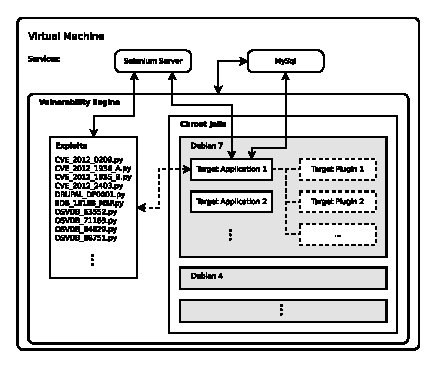
\includegraphics[scale=1.17]{system_diagram.eps}
\end{center}
\caption{System Diagram}
\end{figure}


\subsection{Engine}
The {\bf Engine} drives the environment setup, tear-down, and exploitation process. The engine was created to abstract away details so that researchers can easily run exploit scripts without having to worry about getting the target application running every time. \par
The vulnerability engine controls the actions of a given exploit, and ensures that the proper target environment, application, and application plugins are properly setup in the {\tt chroot} environment. The role of the engine is illustrated in the two use-cases. For example, following relevant lines in Use-Case 1:
\begin{description}
  \item[Line 5] {\tt \footnotesize    engine = Engine(Exploit(), config)} \\ A new engine instance is constructed with an exploit instance and system configuration as arguments.
  \item[Line 6] {\tt \footnotesize     engine.startup()} \\The engine creates a {\tt chroot} environment on the host system to which the target application is copied and the pertinent MYSQL databases are established. The setup of the environment is determined by the 'Target' attribute in the exploit instance. 
  \item[Lines 7 \& 9] {\tt \footnotesize engine.xdebug\_autotrace\_on()\\ engine.xdebug\_autotrace\_on()}\\The engine can modify the state of the trace collection in X\_Debug to ensure that we collect only the trace pertinent to the exploitation.
  \item[Line 10] {\tt \footnotesize engine.shutdown()}\\Cleanup unmounts the {\tt chroot} environment and returns the corpus environment back to an un-altered state.
\end{description}



%\begin{figure}[!tp]
%\begin{center}
%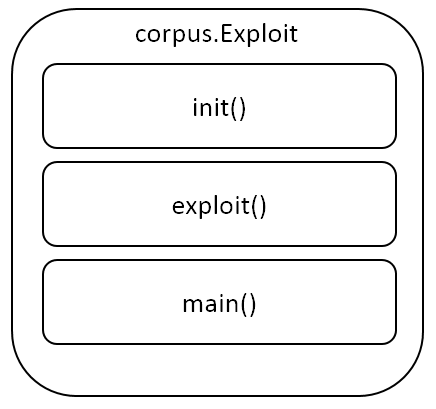
\includegraphics[scale=.5]{Corpus_Exploit.PNG}
%\end{center}
%\caption{Exploit Structure}
%\end{figure}


\subsection{Targets}
   The {\bf Target} module controls all the application targets that the exploits may be applied to.  More specifically, this represents web applications such as WordPress, SimplePHPAgenda, etc. A copy of the target program with a typical configuration, is always loaded before any exploit script is run.  Init scripts are written per application to provide the {\bf Engine} with the proper details for the setup, for example:

\begin{minipage}{\textwidth}
{\tt \footnotesize
%\begin{verbatim}
\begin{lstlisting}
name = "Wordpress 3.3.1"
application_dir_mapping = ...
     [get_path("application"), "/var/www"]
database_filename = get_path("database.sql")
database_name = "wordpress_3_3_1_A"
chroot_environment = "Debian7"
\end{lstlisting}
%\end{verbatim}
} 
\end{minipage}


Some large web applications, such as WordPress, have many plugins that in themselves, have vulnerabilities. Therefore {\bf Target} modules also allow for the inclusion of plugins in the exploit framework.Both targets, and target plugins are resolved against the exploit attributes by the Engine during the setup process. 


\subsection{Exploit}
The {\bf Exploit} class is the superclass for each exploit in the corpus, defining interfaces and attributes that the engine uses to manage the environment and exploitation. The structure of Exploit is designed so that exploits can be written as a concise code statement. Each exploit is simply a subclass of Exploit residing in it's own Python file in which all actions taken by the exploit are clearly visible. In addition, a Query module is provided that will return a set of Exploit instances based on matching against the meta-data specified in the exploit (as shown in the use-cases).\par

This separation accomplishes a step-like approach for getting involved with the corpus, where developing exploits for the corpus is more approachable and quick for novice programmers that wants to contribute and a robust framework that can be understood incrementally for larger contributions to the framework.\par
 
This template ensures that the selenium driver is properly initialized bound to the exploit and makes sure that an exploit script has been defined as well as defines any specific actions on tear-down.\par

The exploit module is annotated by it's attribute dictionary. In it we declare the name, description, references, target, type and wiki page for the exploit by the attributes dictionary.  The name is the technical name specified in one of the online databases of exploits and vulnerabilities mentioned earlier in the paper.  The description is a brief statement of what the exploit is supposed to do, because the name is typically not descriptive enough for a person to understand what type of exploit is being applied.  The Target is the web application target that is being used for the exploit.  The type is the type of exploit being conducted.  The VulWikiPage is the wiki page setup for an author to place auxiliary information about the exploit or script.

Here is an example body of an exploit procedure used for the simplest of XSS attacks.  The entire exploit consists only of instantiating the selenium driver and submitting a post on the WordPress site with the payload: 

\begin{minipage}{\textwidth}
{\tt \footnotesize
%\begin{verbatim}
\begin{lstlisting}
payload = "<a href=\"#\" title=\"XSS http:" \
          "//example.com/onmouseover=eval(" \
          "unescape(/%61%6c%65%72%74%28%31" \
          "%29%3b%61%6c%65%72%74%28%32%29%" \
          "3b%61%6c%65%72%74%28%33%29%3b/." \
          "source))//\">XSS</a>"

driver = self.create_selenium_driver()

driver.get("http://localhost/wordpress/?p=1")
get = driver.find_element_by_id
get("author").send_keys("selenium script")
get("email").send_keys("selenium@python.org")
get("url").send_keys("www.python.org")
get("comment").send_keys(payload)
get("submit").click()
\end{lstlisting}
%\end{verbatim}
}
\end{minipage}

\subsection {Cleanup and maintenance}

Multiple methods that perform cleanup and maintainance are included in BugBox to ensure that results are reproducible. With this in mind, there are many changes that occur in the system through the course the exploit cycle that need to be eliminated. Even changes that would normally seem inocuous, like recording events to a log-file, have the potential to at some point change program behaviour, and should not be allowed. BugBox has seperate methods that maintain the integrity of the target modules the evironments.

Since the {\tt chroot} environments exist on the host machine as simple directories, it is trivial to write scripts for managing them.  Scripts using {\tt rsync} are employed to periodically overwrite the {\tt chroot } jails to maintain the integrity of the operating system. Each exploit is then responsible for managing it's own side-effects on the target application. For instance, many exploits result in the inclusion of an arbitrary file to be executed by the webserver. The exploit superclass provides for a cleanup method to be written when implementing an exploit for exactly these types of vulnerabilities. When defined, the cleanup method is invoked after the successfull application of exploit to restore the target module to it's pre-exploitation state. 


This wrapper class allows the exploit writer to choose whether to display the Firefox browser during exploitation. This feature has proven very useful for debugging exploits, and has lead to quicker turn-around in the exploit development. With the Selenium Driver, one can also orchestrate demonstrations to teach others the principles behind web vulnerabilities.  A setup could entail showing a live feed of tcpdump and the Apache logs on one screen, while in real-time one Firefox process shows the actions taken by an attacker posting a malicious script on a forum, after which the session for an unsuspecting admin in an adjacent Firefox process shows the activation of a CSRF exploit. 

\section {Lessons learned}

In developing BugBox, we learned {\em four} key lessons: Flexibility of environment, visual aids speed up exploit script development, developing a large diverse corpus is quicker with community involvement, quick script verification can increase corpus quality and repeatability of experiments.\par

Having flexibility over choosing the environment in which web applications are installed is a critical factor in corpus development.  The goal of creating a corpus is to create a wide variety of examples, and in doing this we sometimes have to use web applications that are outdated.  Incorporating these web applications into the corpus leads to dependencies on older language versions that have dependencies for different Linux distributions.\par

Exploit script development is a repetitive and necessary process.  We found that in developing the exploit scripts alongside the Selenium visual framework we could more rapidly create exploit scripts.  This increase in productivity is directly correlative to the visual execution monitoring of the scripts allowing developers to efficiently pinpoint errors and enhancing script generation.  \par

In collecting samples for our original corpus we focused on the quantity of samples, but did not emphasize diversity of samples.  In attempting to conduct statistical tests on the corpus we needed a better representative sample.  Taking a community approach for corpus development and streamlining corpus entry allows us and the community obtain a large quantity of data that is diverse and representative.\par

Finally, verification of the vulnerable traces was originally difficult because trace data can be verbose and we did not have scripts to make repeatable results.  By executing the Selenium script, one can visually verify that the exploit is being run and captured correctly in a matter of seconds. 

\section{Future work}
We plan to implement additional features for controlling trace collection through cookie manipulation via XDebug. This will reduce the collection of insignificant interactions and provide a more refined break-down of the exploitation process since traces can be grouped by HTML request. For each exploit currently in the corpus, there is no standard for the payload used in the attack. Since studies on intrusion detection or prevention systems may be sensitive to the payload type and encoding, researchers may desire finer-grained control over this property. The Metasploit Framework has a  robust system for managing exploits along with their payloads and encodings and serves as a model for implementing this.

We also plan to make BugBox available to the security community in the near future. BugBox is designed to work on the Debian GNU/Linux and compatible distributions.  The framework will be distributed under an open-source license, both as as a self-contained virtual machine and as a package that can be installed on an existing system. The machine must have sufficient storage (roughly 4 GB per OS environment, and up to 2 GB for the application, engine, and exploit sources), with access rights to use run Linux {\tt chroot} jails.  Dependencies for the BugBox host system include MySQL, Selenium Server, \texttt{debootstrap}. Community contributions will be key to building a corpus of sufficient size, and we also intend to deploy a wiki allowing contributers to download, submit and discuss BugBox exploit and target modules. Because the corpus is composed entirely of open-source applications, target modules will be distributed under the application's respective license.

\section*{Acknowledgments}

The authors thank the United States Office of Naval Research for its support for this research.

{\footnotesize \bibliographystyle{acm}
\bibliography{ref}}

\end{document}
